%!TEX root = ../thesis.tex
\chapter{Experiments}
In this chapter, both proposed heterogeneous pc-stable algorithm approaches are evaluated. Furthermore, two different systems are used for the evaluation to elaborate the hardware dependency of the heterogeneous version.

\section{Setup}
The dataset the experiments use for computation is based on the dataset used in the experiments of Perscheid et al. \cite{perscheidIntegrativeGeneSelection2018}. The dataset is taken from The Cancer Genome Atlas (TCGA) \cite{weinsteinCancerGenomeAtlas2013}. Genes with more than 30\% missing values are filtered out. The remaining data is normalized and log-transformed. The original dataset consists of 55 573 variables. While the run-time of the PC stable algorithm grows exponentially with the variable count, subsets of the dataset are used for evaluation. The subset sizes chosen for the evaluation are 1000 variables, 10 000 variables, and 45 000 variables. The 1000 variables dataset is used to represent small datasets and will be called TCGA-1000. The 10 000 variables dataset is a large dataset that does not fill the memory of the system's GPU. The 45 000 variables dataset is therefore used to show the effects of GPU memory overflow on the algorithms execution time in this evaluation.

\begin{figure}[h]
  \caption{System 1 Structure - Delos}
  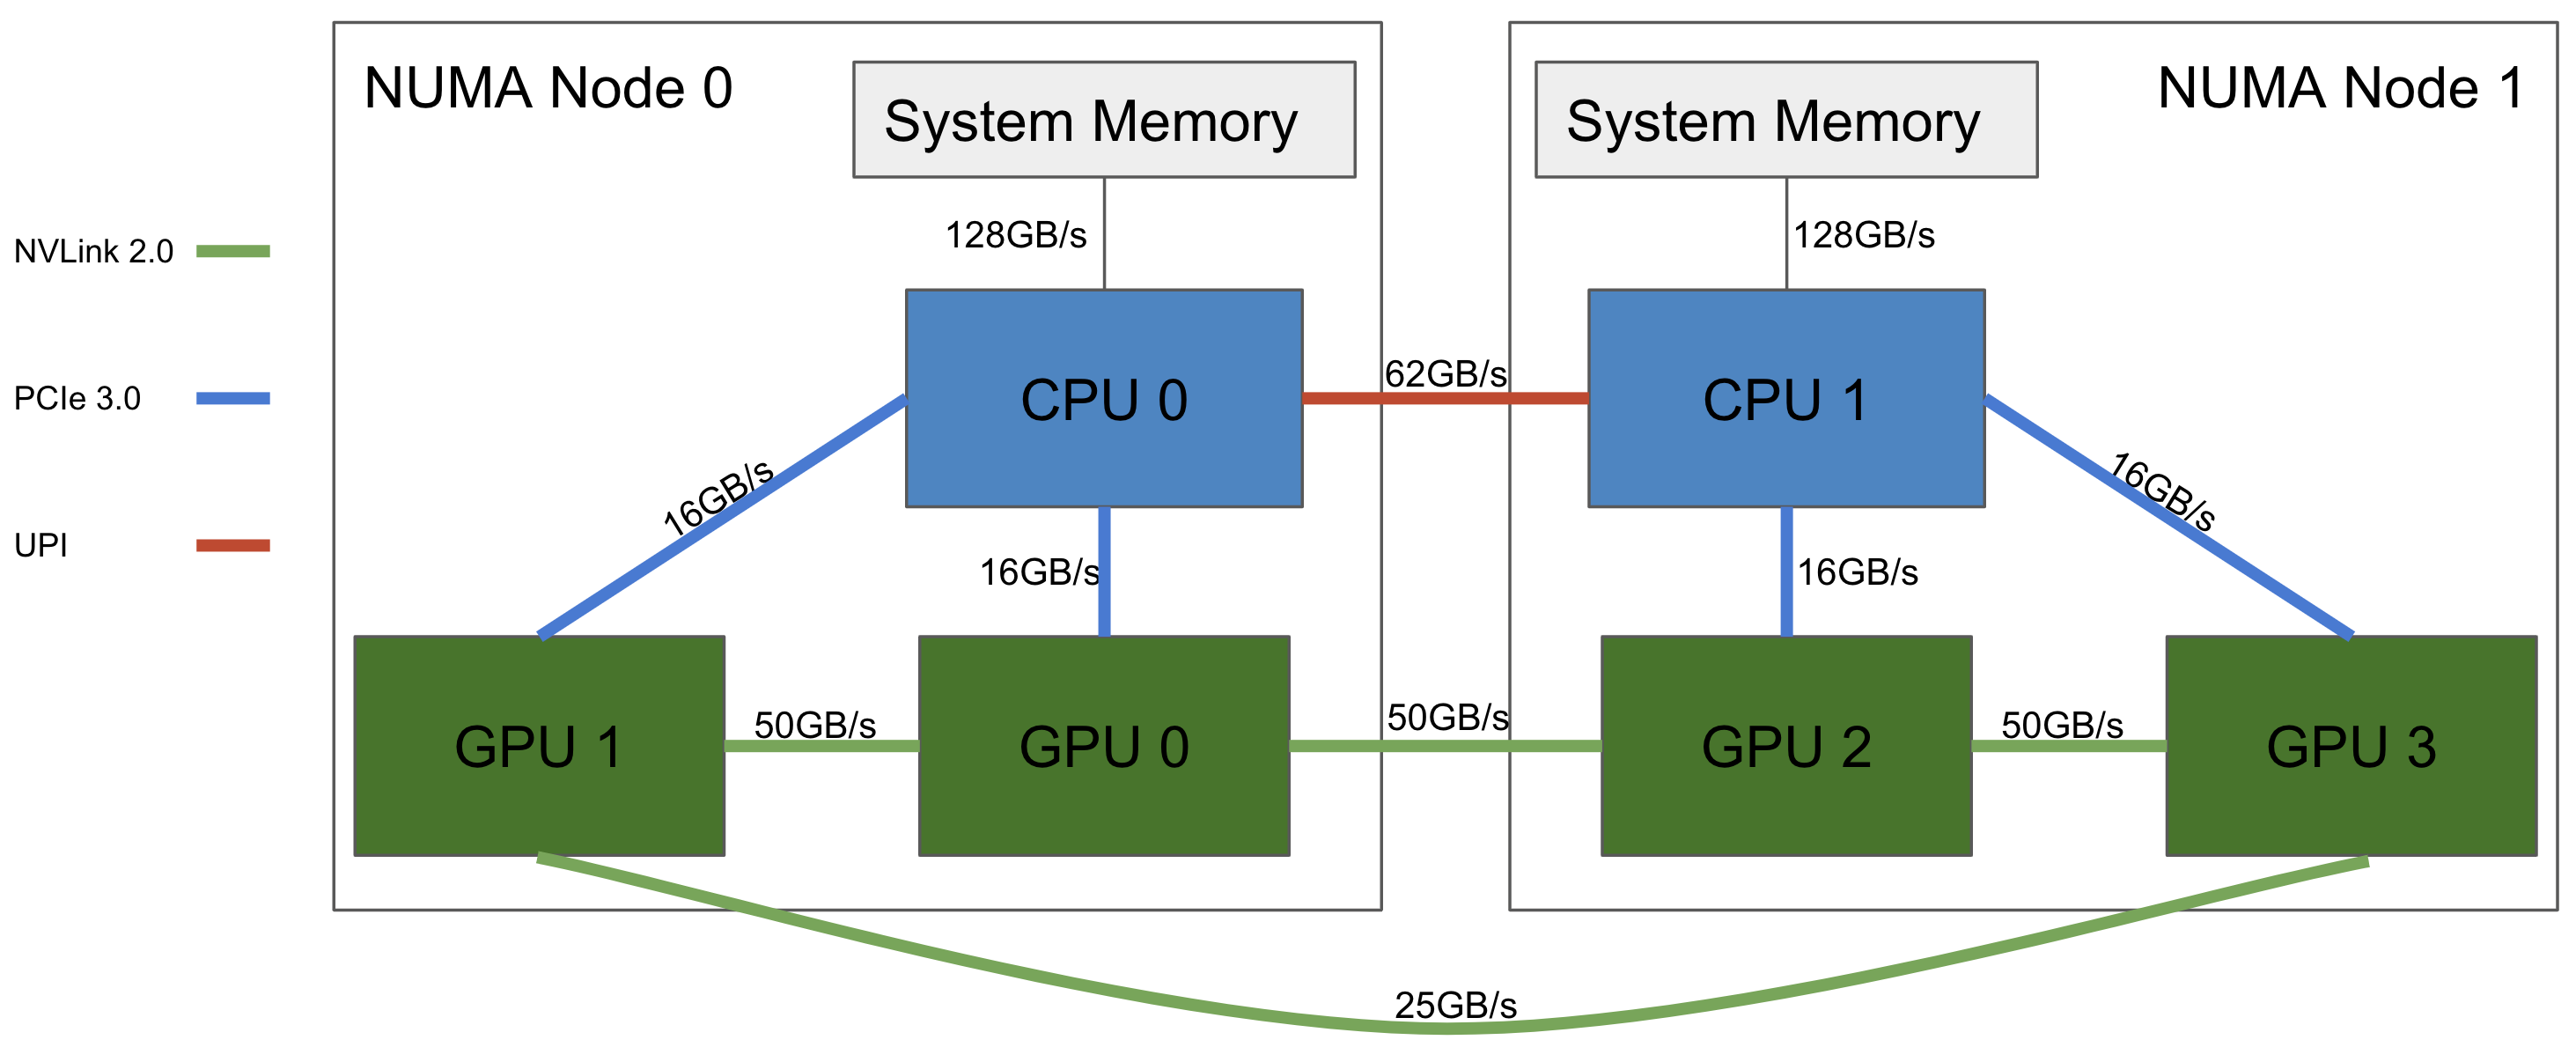
\includegraphics[width=\textwidth]{figures/delos_system_arch.png}
  \centering
  \label{fig:delos_arch}
\end{figure}

Two different systems are used for the evaluation. One system, which will be called Delos \ref{fig:delos_arch} in the following, consists of 4 Nvidia Tesla V100 GPUs with each 32GB of SXM2 memory and 2 Intel Xeon Gold 6148 CPUs with each 755GB of DDR4 memory. The Tesla V100 GPU clock rate is 1,53 GHz. It contains 80 Streaming Multiprocessors which each can execute a maximum of 2048 threads concurrently \cite{NVIDIATESLAV1002017}. The Intel Xeon Gold 6148 has 20 cores with a clock rate maximum of 3,70 GHz. Each core has two so-called hyper threads so that the CPU can execute 40 threads concurrently.

\begin{figure}[h]
  \caption{System 2 Structure - AC922 \cite{ganesannarayanasamyPowerAIDeepDive12:39:24UTC}}
  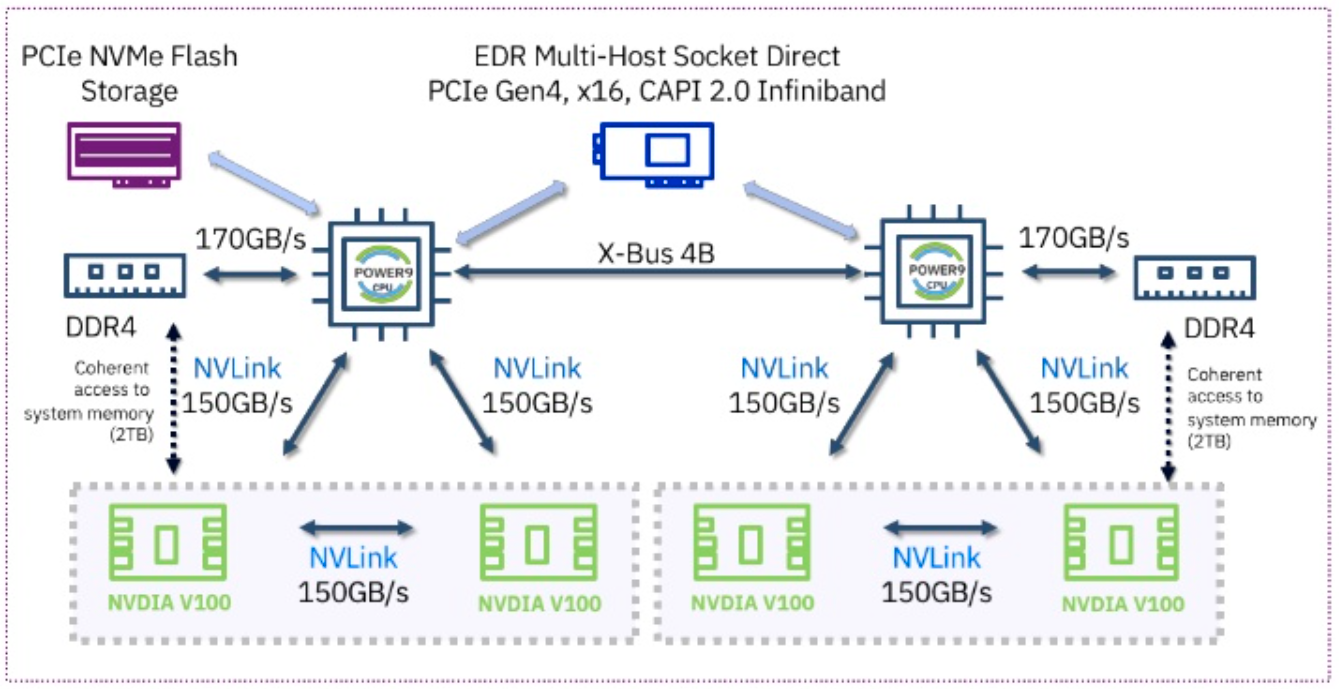
\includegraphics[width=\textwidth]{figures/ac922_system_arch.png}
  \centering
  \label{fig:ac922_arch}
\end{figure}

The second system, which will be called AC922 \ref{fig:ac922_arch} in the following, is a high-performance computing system developed in collaboration with IBM and Nvidia \cite{caldeiraIBMPowerSystem}. It incorporates the same GPUs as the Delos system (4xNvidia Tesla V100) and two IBM Power9 processors. Each Power9 processor has 16 cores with a clock rate maximum of 4 GHz, which, by using SMT4 multithreading, can execute 64 threads concurrently. 256GB DDR4 RAM is connected to each CPU.

Through the collaboration of IBM and Nvidia, the interconnect between a CPU and GPU in this system is NVLINK \cite{NVLink2021, zargesEvaluationOnNodeGPU} with a bandwidth of 150GB/s in contrast to the Delos PCIe 3.0 16GB/s interconnect. NVLINK is also faster latency wise \cite{liEvaluatingModernGPU2020}. The latency and throughput differences of both systems allow evaluating bottlenecks regarding interconnect speed in this heterogeneous computation scenario.
Furthermore, the collaboration brings other features which a heterogeneous computing application can benefit from, such as Adress Translation Services \cite{ibmpower9nputeamFunctionalityPerformanceNVLink2018} unifying the GPU and CPU page table, native atomics support for system-wide accessible memory and direct GPU memory access by the CPU \cite{UNIFIEDMEMORYP9}.

The following experiments only use one GPU for execution, even if the proposed algorithm can be executed on multiple GPUs at once. Therefore parameters, such as GPU-GPU memory handling and interconnect technology, do not influence the CPU-GPU computation results. Some benchmarks are pinned to the NUMA node closest to the executing GPU to limit interconnect effects not related to the direct CPU-GPU connection. Both systems' CPUs are directly connected to two GPUs, which means using only half the cores and memory while NUMA pinned. The largest dataset being used with the size of 36GB$\sim$ will not be the limiting factor for the CPU's associated memory of 755GB on Delos and 256GB on AC922. On the other hand, 36GB$\sim$ of data will fill the GPU's memory of 32GB which is intentional behavior as said above.

The following table shows the tools and libraries used for the experiments:
\begin{table}[h!]
  \centering
  \begin{tabular}{||c | c||} 
   \hline
   Delos & AC922 \\ [0.5ex] 
   \hline\hline
   GCC 8.4.0 & GCC 8.3.1 \\
   CUDA 11.3 & CUDA 11.3 \\ 
   CMake 3.20.2 & CMake 3.20.2 \\
   Armadillo 10.5.1 & Armadillo 10.5.1 \\
   Boost 1.65.1 & Boost 1.76.0 \\ [1ex]
   \hline
  \end{tabular}
  \caption{Tools and libraries and their versions used in the experiments}
  \label{table:libversions}
\end{table}

Further the following flags were passed to GCC on the systems:
\begin{itemize}
  \item Delos: -O3 -DNDEBUG -march=native -mtune=native
  \item AC922: -O3 -DNDEBUG -flto -fpeel-loops -funroll-loops -ftree-vectorize -ffast-math -mcpu=power9 -mtune=power9
\end{itemize}
The flags used on the AC922 system are recommended by IBM for optimized binaries \cite{LinuxIBMPower}. NVCC, the Nvidia CUDA compiler, gets passed the same flags on both systems (-O3 -DNDEBUG -lineinfo). Additionally, CMake automatically sets the correct flags to compile for best optimization on the V100 architecture.

\section{Benchmarks}
For each system, basic experiments for both approaches are done first to determine the relevance and effectiveness of those approaches. To analyze hardware-specific effects on the experiments, more detailed benchmarks are done later, such as tests with a modified thread count used for the CPU execution.
The first approach, which is called pre-balanced, will be tested and compared to the GPU-only execution of the algorithm. Additionally, the effect of migrating edges after each level and pinning the execution to some NUMA node is tested as well.

The same tests are then done for the workstealing approach, where a test for atomic usage is added since atomics are not necessary for this approach and only used so that edges are not processed twice.

Those described experiments are done on both the Delos system and the AC922 system. Each test relying on the dataset with 1000 variables is executed five times, and for the final result, the mean of all results is calculated. On the Delos system, further experiments to evaluate the scalability of the approaches are done using large datasets, as said above.

\subsection{Benchmarks Delos}
\begin{table}[H]
  \centering
  \begin{tabular}{||c | c | c | c||} 
   \hline
    & Execution time (ms) & $\Delta$ & $\Delta$ speedup in \% \\ [0.5ex] 
   \hline\hline
   GPU-only & 16290.8 & 0 & - \\
   Pre-Balanced & 15853.8 & -437 & 2,68 \\ 
   No post level migrations & 15821.8 & -469 & 2,96 \\
   NUMA node pinned & 16839.6 & 548,8 & -3,36 \\ [1ex] 
   \hline
  \end{tabular}
  \caption{Pre-Balanced execution time results (Delos)}
  \label{table:preb_delos}
\end{table}
The first experiments using the pre-balanced approach seen in \ref{table:preb_delos} show that there is a slight performance boost of 2,9\% in comparison to the GPU-only variant possible. While pinning the NUMA node, there is even a slow down seen, which tells us two things: First, the missing processing power of the lost cores while pinning the execution is missing, and more cores should help in speeding up the execution. Second, the interconnect bottleneck does not hit the performance in a meaningful way when edges of different rows are processed by GPU and CPU, supported by the little to no effect of migrating edges after level execution. Additionally, the count of rows placed on the CPU by the load balancer had to be tuned carefully for the best performance. The row count balanced on the CPU is 14 rows in level one and two and 8 rows in level three and four, which is small compared to the maximum of 1000 rows.

This volatility makes tuning the pre-balanced approach hard, especially for large datasets where the PC stable algorithm can execute for hours or days. Multiple tuning executions might not be feasible in such situations because this threshold might change a lot for different datasets, which could lead to more sparse rows.

\begin{table}[H]
  \centering
  \begin{tabular}{||c | c||} 
   \hline
    & Execution time (ms) \\ [0.5ex] 
   \hline\hline
   GPU-only & 16290.8 \\
   Workstealing & 15796.8 \\ 
   Workstealing without postponed edge migrations & 15892.2 \\
   Workstealing without atomics & 23551.0 \\
   Workstealing NUMA pinned & 16266.4 \\ [1ex] 
   \hline
  \end{tabular}
  \caption{Workstealing execution time results (Delos)}
  \label{table:workst_delos}
\end{table}
Experiments with the workstealing approach seen in \ref{table:workst_delos} show a 3,1\% performance boost in comparison to the GPU-only execution, which is similar to the pre-balanced approaches result, even if there should be dynamic scheduling overhead. Postponing the migration of the edge deletion does not impact the execution time, whereas the benchmark without atomics shows a slowdown of $\sim$33\ in comparison to using atomics. The reason for the slowdown while not using atomics is presumably because tasks are processed multiple times and changes to the flags annotating tasks that are being processed have to be migrated via pages between the processors.

Comparing the pre-balanced approaches and the workstealing approaches results, both seem to be similarly effective for speeding up the pc-stable variant. Still workstealing and dynamic scheduling is more flexible and does not need to be tuned for the dataset being used. Due to the flexibility, further tests on the Delos system are done using the workstealing approach.

\begin{figure}[h]
  \caption{Testing the CPU side parallelizability of the workstealing approach on Delos. The approach does no scale well with multiple cores}
  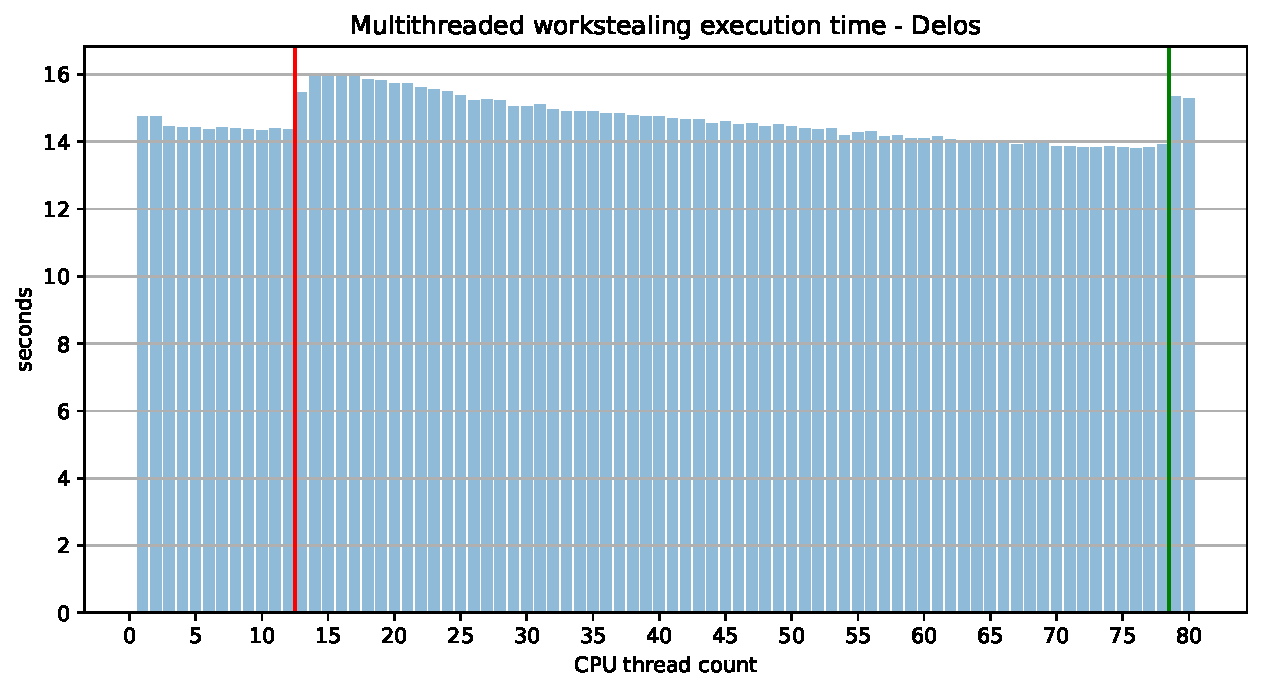
\includegraphics[width=\textwidth]{figures/threaded_wsteal.pdf}
  \centering
  \label{fig:wstealing_threaded_delos}
\end{figure}

The implementation of the CPU execution is parallelized with OpenMP, a library that allows easy tuning of the thread count that is spawned for execution. In the following experiment, the parallelizability of the CPU execution is tested \ref{fig:wstealing_threaded_delos}.
The peack at 80 threads is to be expected, because there is also a main thread, used for orchestration, and one thread per GPU, used for GPU synchronization, running. With 80 plus 2 threads running there is not enough execution units available to have all of them running without collisions. Therefore the maximum number of threads, that should be used is 78.

While a performance boost can be seen for additional threads spawned, there is another peak of execution time at around 20 threads. This peak might be explained by bad optimization, which could be an interconnect bottleneck hit with the two NUMA nodes involved or the system-wide synchonization through atomics. 78 thread execution is the fastest, but not by far and therefore might not be suitable in comparison to one thread in energy efficient environments. The speedup of 78 threads workstealing to GPU-only is $\sim$16,6\%.

\begin{table}[H]
  \centering
  \begin{tabular}{||c | c | c||} 
   \hline
   Variable count & 1 thread speedup factor & 78 threads speedup factor \\ [0.5ex] 
   \hline\hline\hline
   1000 & 1,11x & 1,17x \\
   10 000 & 0,95x & 0,96x \\ 
   45 000 (only level 0 and 1) & 1,06x & 6,61x \\ [1ex] 
   \hline
  \end{tabular}
  \caption{Workstealing execution time results (Delos)}
  \label{table:workst_delos_scaling}
\end{table}

Looking at the scalability of the workstealing approach by running benchmarks on larger datasets it can easily be seen, that the approach does not scale well. Because at 10 000 variables there is even a slowdown. The reason for this slowdown is that the data migration between the CPU and the GPU rises with more variables to be randomly accessed and the CPU-GPU interconnect is limited in its througput. More variables also produce more row length peaks, which are less likely to be an outlier, because of the higher possibility of occuring peaks.
The GPU-only execution is faster, due to the more balanced data and the better memory access times.

While the dataset based on 10 000 variables does not exhaust the memory associated with the GPU, the 45 000 does. By exhausting the GPU memory, the CUDA runtime has to swap memory in and out while accessing, because there is always a part of the dataset, which cannot be held in memory. This swapping process is usually slow, because the CPU-GPU interconnect is used, and does get triggered often if there is some random access pattern.

The CPU still holds the whole data in system memory and is able to access the data fast. The heterogeneous computing approach is 6,61 times faster then the GPU-only variant, because the memory overflown GPU is slower in this case and the CPU can help more in relation to the other cases.
Since the raw computing power is the most important part about the CPU in this scenario, using more threads speeds the computation up as well.

\begin{figure}[h]
  \caption{Comparing the level-wise speedup factor of the pre-balanced and workstealing approach to GPU-only execution}
  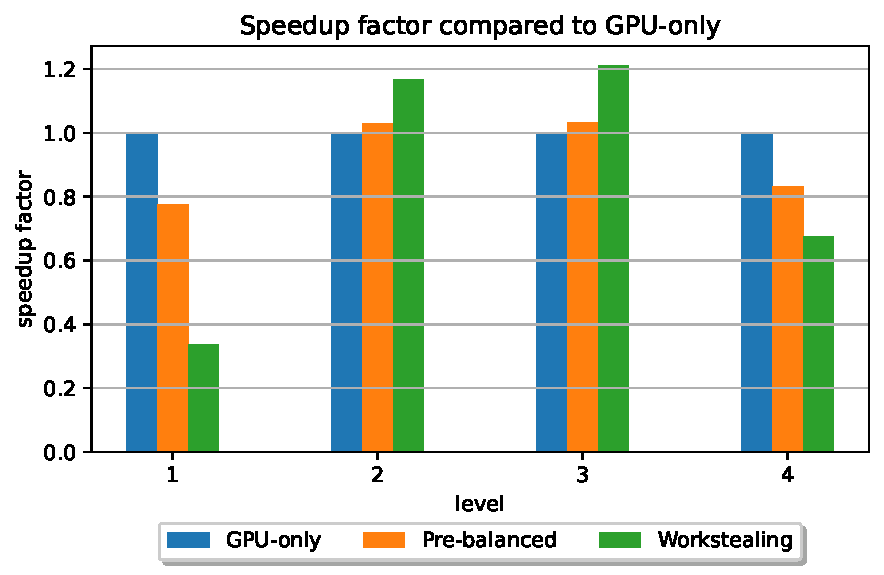
\includegraphics[width=\textwidth]{figures/levelwise.pdf}
  \centering
  \label{fig:levelwise_delos}
\end{figure}

By comparing the speedup level-wise in \ref{fig:levelwise_delos} it is clear that level 2 and 3 are impacted by the heterogeneous computing speedup through the CPU. Level 1 and 4 are slower than GPU-only when executed heterogeneously because there are less to none execution-time outlier tasks in the data, that can be placed on the CPU. In level 2 and 3 there are larger and more performance impacting outlier tasks. The influence of level 1 and 4 is negligible, due to the small share of 1\% in the execution time. Nevertheless, the best performance is achievable through executing only level 2 and 3 via heterogeneous computing.

Interestingly the most tasks are stolen in level 2 by the CPU. While the CPU steals around 90 000 tasks in level 1 where the additional help of the CPU slows the execution, the CPU steals around 4000 tasks in level 2 and 1000 in level 3. This is to be expected, because tasks in higher levels are slower on average and the CPU takes the longest tasks on purpose. This difference in processed tasks on the CPU supports the argumentation, that in level 3 and 4 more outliers are done on the CPU, which take generally longer.

\subsection{Benchmarks AC922}
After exploring both approaches on the Delos system, a further look into the bottleneck of the CPU-GPU interconnect is evaluated by doing comparable benchmarks on the AC922, whose interconnect is faster by relying on NVLINK in contrast to Delos, which relies on PCIe. Native system-wide atomics should also show in the workstealing benchmarks.
While the GPU built into both systems is the same Nvidia V100 GPU, the built-in CPUs are different and might impact the benchmarks.

While the Intel Xeon CPU included in the Delos system is x86\_64 architecture based, the Power9 CPU, which is included in the AC922 system, is based on the ppc64le architecture. Through the different architectures of both CPUs, different optimizations are done, which can influence execution times \cite{AnalysisX86Vs}.


% - Explain dataset used for testing (TCGA)
%   - Variable size
%   - how sampled
%   - paper (perscheid etc)
% - Show delos as a testing machine
%   - Intel Xeon 
%   - Nvidia  V100
%   - specs
%   - numa nodes
% - Show AC922
%   - Explain why power9 + V100 special
%   - ATS: Malloc is enough
%   - Faster interconnect NVLINK
%     - Comparison between interconnects
%   - Other pros : atomics etc
%   - Explain why this should affect my performance
%   - Compare Power9 to Intel Xeon
% - Show iteration measurements per level
%   - show how many tests and iterations have to be done

% - Measurements of GPU only Code

% - Measurements of Pre-balanced
%   - With, without migrating edges
%   - Different thresholds
%   - Different Dataset sizes
%   - Different omp scheduling methods
%   - Pinning on NUMA nodes
%   - Delos vs AC922
% - Measurements of Workstealing
%   - With, without migrating edges
%   - Different Dataset sizes
%   - Pinning on NUMA nodes
%   - Delos vs AC922

% - Measurements with different Datasets
%   - Iterations
%   - Workstealing Numa 0
%   - Prebalanced
%   - GPU only
